\section{Linux and GCC}
Nous allons ici réaliser les mêmes étapes que précédemment mais cette fois dans un environnement Linux. Nous nous plaçons donc sur un poste Ubuntu 14.04 LTS - 64 bits.
\subsection{Crashing your program}
En exécutant le premier programme avec en paramètre \enquote{\%s}, nous obtenons les sorties suivantes :
\begin{figure}[H]
  \centering
  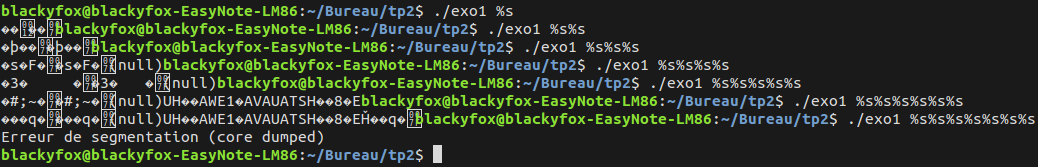
\includegraphics[width=.9\textwidth]{img/c1.png}
  \caption{Résultat de l'exécution du premier programme}
  \label{img:li:1}
\end{figure}
Comme nous pouvons le constater, il est nécessaire de donner 7 fois le paramètre \enquote{\%s} au programme pour que celui-ci rencontre une erreur.\\
Il est possible d'utiliser \textit{Valgrind} afin de mieux comprendre pourquoi cette erreur a eu lieu :
\begin{figure}[H]
  \centering
  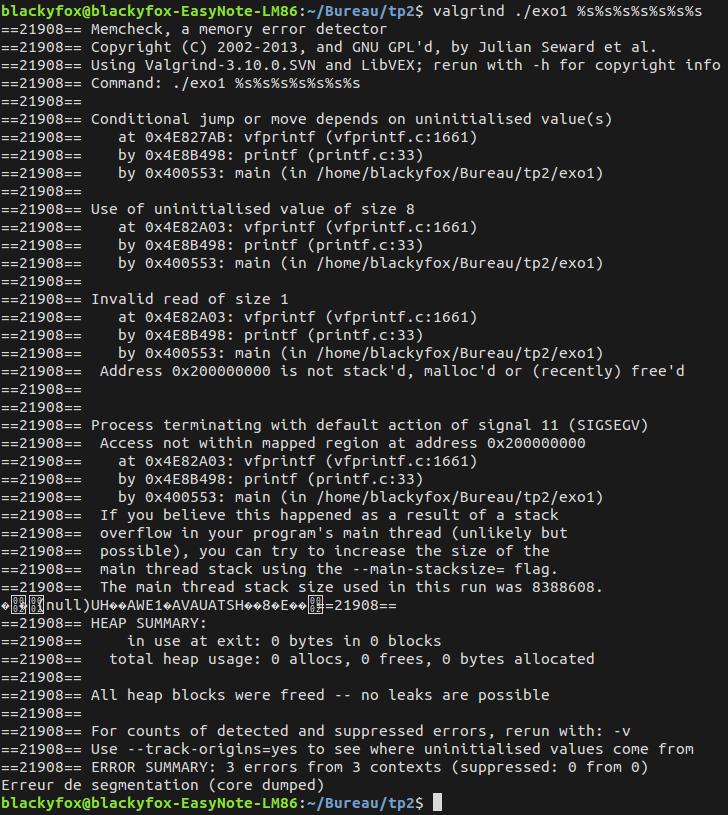
\includegraphics[width=.9\textwidth]{img/c2.png}
  \caption{Résultat de l'exécution du premier programme avec \textit{Valgrind}}
  \label{img:li:2}
\end{figure}
Ainsi, comme précédemment, nous pouvons remarquer que comme vu dans le point \ref{crash} que le programme essayer d'accéder à une zone mémoire qui lui est interdite. Ainsi, le programme ne pouvant pas lire la donnée en mémoire s'arrête.

\subsection{Viewing the stack}

Tout comme pour le point \ref{stack}, nous allons ici retrouver des adresses mémoire en donnant en argument \enquote{\%08x} à notre premier programme :
\begin{figure}[H]
  \centering
  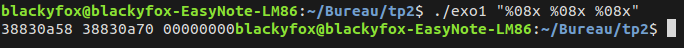
\includegraphics[width=.9\textwidth]{img/c3.png}
  \caption{Résultat de l'exécution du premier programme avec \enquote{\%08x} en argument} 
  \label{img:li:3}
\end{figure}
Le premier \enquote{\%08x} va nous permettre de retrouver l'adresse mémoire d'$EBP$, ici égale à $38830A56$.\\
Cependant, nous ne retrouvons pas la valeur de $EIP$ dans le second argument. En effet, nous savons que $EIP=EBP+4$. Ainsi, nous devrions retrouver l'adresse $38830A5A$ en seconde adresse de sortie. Nous avons cependant ici l'adresse $38830A70$.\\
Nous pouvons donc conclure que nous le compilateur GCC n'agit pas de la même façon que dans notre test précédent, sur la machine virtuelle de Windows XP.

\subsection{Overwriting the memory}

Ici encore, nous pouvons retrouver le même type de sortie que sur la machine virtuelle de Windows XP (c.f. \ref{over}) :
\begin{figure}[H]
  \centering
  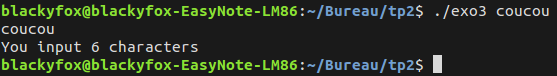
\includegraphics[width=.9\textwidth]{img/c4.png}
  \caption{Résultat de l'exécution du troisième programme} 
  \label{img:li:4}
\end{figure}
Ainsi, la fonction \textit{printf} va ici aussi compter le nombre de caractères écrit puis stocker cette valeur en mémoire.\\
Il est possible de vérifier cela en utilisant \textit{Valgrind} :
\begin{figure}[H]
  \centering
  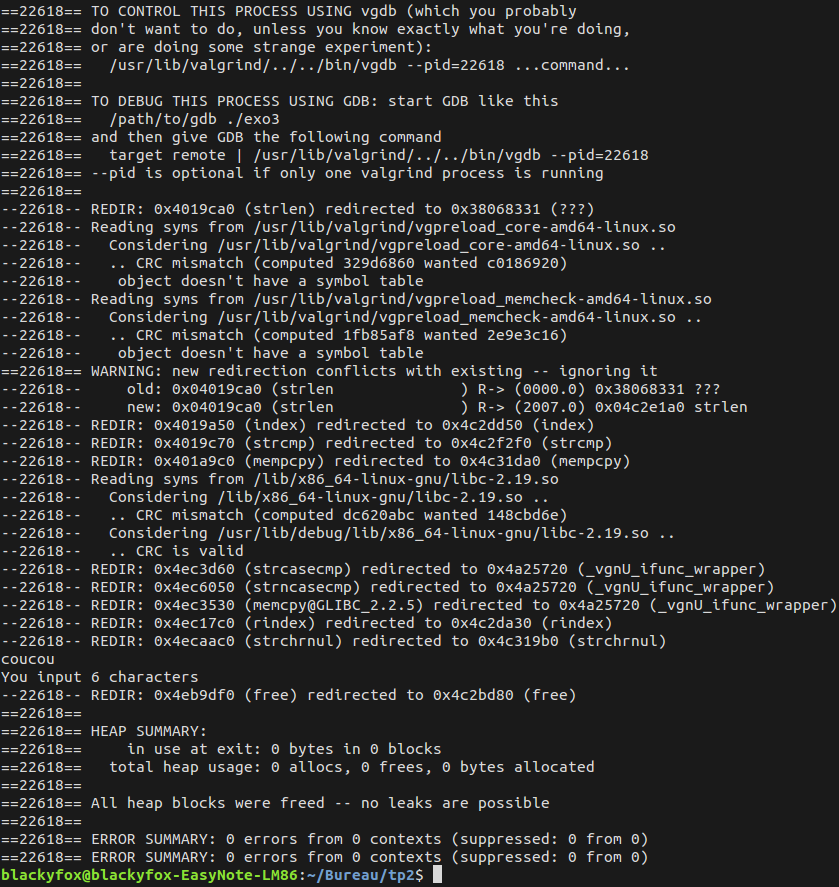
\includegraphics[width=.9\textwidth]{img/c5.png}
  \caption{Résultat de l'exécution du troisième programme} 
  \label{img:li:5}
\end{figure}
Comme le montre la figure \ref{img:li:5}, nous pouvons remarquer que le programme utilise la fonction \textit{strlen}. C'est en effet cette dernière qui va permettre à la fonction \textit{printf} de connaître la taille des données écrites. On va ensuite retrouver l'utilisation de la fonction \textit{mempcpy} qui va permettre au programme de copier la valeur comptée dans la variable \textit{byte} du programme.

\section{Windows 7 and Visual Studio}